\documentclass[12pt,a4paper]{article}

% Margins.
\setlength{\oddsidemargin}{0in}
\setlength{\evensidemargin}{0in}
\setlength{\headheight}{12pt}
\setlength{\headsep}{0pt}
\setlength{\topmargin}{-60pt}
\setlength{\textwidth}{6.5in}
\setlength{\textheight}{10.75in}

\usepackage{amsmath}
\usepackage{float}
\usepackage{graphicx}
\usepackage[hyphens]{url}
\usepackage{hyperref}	% Clickable links to figures, references and urls.
\usepackage{datetime}
\usepackage{longtable}

% Drawing.
\usepackage{pgf}
\usepackage{tikz}
\usepackage{amssymb}  % Tick mark
\usepackage{textcomp} % Cross

% Listings for formatting code.
\usepackage{listings}
\usepackage{textcomp}
% General options.
\lstset{breaklines=true, basicstyle=\small\ttfamily, tabsize=4, numbers=left, stepnumber=1, frame=single, showstringspaces=false, upquote=true}
% C++ specific high-lighting. Comments are 50/50 shades of green/black and strings coloured with 60/40 red/black mixture.
\lstset{language=[ISO]C++, commentstyle=\color{green!50!black}, keywordstyle=\color{blue}, stringstyle=\color{red!60!black}}

%opening
\title{Introduction to Computing\\Lab 13\\C--Strings Practice}
\author{Moomal Bukhari\and Attique Dawood}
\date{May 26, 2015\\[0.2cm] Last Modified: \today, \currenttime}
\begin{document}
\maketitle
\section{What are Strings?}
Simple answer: character arrays are called C--strings (or simply string). A bunch of characters most often only make sense if they form words. And words only make sense if they are part of a sentence. Essentially, character arrays are used for storage of words, sentences or the like.
\section{Initialisation at Declaration}
Character arrays have an additional way of initialisation, in addition to other array initialisation methods. Without specifying size, a char array is assigned a string at declaration. In this case, compiler automatically allocates space for array. To print the contents of an array using \texttt{cout}.
\begin{lstlisting}
char myName[] = "abc";
cout << myName;
Output:
abc
\end{lstlisting}
\section{The \texttt{NULL} Character}
Length of words and sentences is not fixed. When strings are stored in character arrays they may not take up the whole space. You might ask the question, when using \texttt{printf} how does the compiler know when the string ends? The answer is that every string ends (or must end) with a \texttt{NULL} character (or \verb|`\0'| in ASCII). In above example, \texttt{myName} was allocated 4 bytes by compiler to end the string with a \verb|`\0'| character. Built-in string functions like this one automatically append \verb|`\0'| at the end of a string. In case you are working or manipulating character arrays directly, then you must take care of \verb|`\0'| yourself.
\section{Length of String}
Length of a string does not include \verb|`\0'|. It only counts the total number of characters before \verb|`\0'|. The \textbf{size of array} containing string and \textbf{length of string} are two different things. In the code segment below, size of array is 10 and length of stored string is 3.
\begin{lstlisting}
char myName[10];
myName[0] = 'a';
myName[1] = 'b';
myName[2] = 'c';
myName[3] = '\0'; // Terminating NULL character.
cout << myName << endl;
Output:
abc
\end{lstlisting}
\section{String Input}
Strings can be input using either \texttt{cin} or \texttt{getline} functions. \texttt{cin} cannot input spaces so \texttt{getline} should be used if input string contains spaces.
\begin{lstlisting}[caption={String Input}]
char Name1[10];
char Name2[10];
cin >> Name1;
cin.getline(Name2, 10); // '10' specifies the maximum number of characters including NULL character. User may enter 9 or less characters.
\end{lstlisting}

Care should be taken when entering strings. The total number of characters must not exceed the size of array. In addition maximum number of characters must be 1 less than array size for a terminating \verb|`\0'|.
\begin{lstlisting}
char CourseName1[10] = "Physics";
char CourseName2[10] = "Programming for Engineers I"
char CourseName3[10] = "Calculus I";

Physics                     // Correct input, string length=7.
Programming for Engineers I // WRONG! Input exceeds size of array.
Calculus I                  // WRONG! No space for '\0', string length=10.
\end{lstlisting}
\begin{figure}[H]
\centering
\begin{tikzpicture}
	\def \displacement {0.0cm}
	% Writing 'CourseName1'
	\draw (-1.5cm,\displacement+0.3cm) node {\textsf{CourseName1:}};
	% Drawing boxes.
	\foreach \x in {0.0cm, 1.0cm, 2.0cm, 3.0cm, 4.0cm, 5.0cm, 6.0cm, 7.0cm, 8.0cm, 9.0cm}
		\draw[thick] (\x, \displacement) rectangle (\x+1.0cm, \displacement+0.6cm);
	% Writing things in boxes.
	\foreach \x/\y in {0.0cm/P, 1.0cm/h, 2.0cm/y, 3.0cm/s, 4.0cm/i, 5.0cm/c, 6.0cm/s, 7.0cm/NULL, 8.0cm/X, 9.0cm/X}
		\draw (\x+0.5cm,\displacement+0.3cm) node {\texttt{\y}};
	% Tick.
	\coordinate [label=above:{\Huge \checkmark}] (Tick) at (10.5cm,\displacement-0.1cm);

	\def \displacement {-0.8cm}
	% Writing 'CourseName2'
	\draw (-1.5cm,\displacement+0.3cm) node {\textsf{CourseName2:}};
	% Drawing boxes.
	\foreach \x in {0.0cm, 1.0cm, 2.0cm, 3.0cm, 4.0cm, 5.0cm, 6.0cm, 7.0cm, 8.0cm, 9.0cm}
		\draw[thick] (\x, \displacement) rectangle (\x+1.0cm, \displacement+0.6cm);
	% Writing things in boxes.
	\foreach \x/\y in {0.0cm/P, 1.0cm/r, 2.0cm/o, 3.0cm/g, 4.0cm/r, 5.0cm/a, 6.0cm/m, 7.0cm/m, 8.0cm/i, 9.0cm/n}
		\draw (\x+0.5cm,\displacement+0.3cm) node {\texttt{\y}};
	% Cross.
	\coordinate [label=above:{\Huge \texttimes}] (Cross1) at (10.5cm,\displacement-0.1cm);

	\def \displacement {-1.6cm}
	% Writing 'CourseName3'
	\draw (-1.5cm,\displacement+0.3cm) node {\textsf{CourseName3:}};
	% Drawing boxes.
	\foreach \x in {0.0cm, 1.0cm, 2.0cm, 3.0cm, 4.0cm, 5.0cm, 6.0cm, 7.0cm, 8.0cm, 9.0cm}
		\draw[thick] (\x, \displacement) rectangle (\x+1.0cm, \displacement+0.6cm);
	% Writing things in boxes.
	\foreach \x/\y in {0.0cm/C, 1.0cm/a, 2.0cm/l, 3.0cm/c, 4.0cm/u, 5.0cm/l, 6.0cm/u, 7.0cm/s, 8.0cm/ , 9.0cm/I}
		\draw (\x+0.5cm,\displacement+0.3cm) node {\texttt{\y}};
	% Cross.
	\coordinate [label=above:{\Huge \texttimes}] (Cross2) at (10.5cm,\displacement-0.1cm);
\end{tikzpicture}
\end{figure}
The solution in this case would be to increase the size of arrays for course 2 and course 3 so they can hold the input strings.
\section{String Manipulation Functions}
String manipulation functions are included in the \verb|<cstring>| header file. 
\begin{table}[H]
\begin{center}
\vspace{0.3cm}
	\begin{tabular}{lp{5cm}p{5cm}}
	\hline \hline
		\textbf{Function} \rule{0pt}{2.6ex} & \textbf{Description} & \textbf{Usage}\\
		\hline
		\verb|strlen()| \rule{0pt}{2.6ex} & Find length of a string & \verb|int len = strlen(str)|\\
		\verb|strcpy()| & Copies str2 into str1 & \verb|strcpy(str1, str2)|\\
		\verb|strcmp()| & Compares two strings. If strings match then 0 is returned. & \verb|if(strcmp(str1,str2)==0)| \verb|    cout << "match";|\\
		\verb|strcat()| & Concatenate str2 onto str1 & \verb|strcat(str1, str2)|\\
		\verb|strrev()| & Reverses string & \verb|strrev(str)|\\
	\hline \hline
	\end{tabular}
\end{center}
\label{Useful string functions}
\caption{Useful string functions}
\end{table}
\section{Exercise}
Implement the following without using library functions.
\subsection{Question No. 1:} Input a string of arbitrary size. Determine the length of this string.
\subsection{Question No. 2:} Take two arrays. Input a random string in one array. Copy this string into second array.
\subsection{Question No. 3:} Take two strings. Check if the strings match.
\end{document}
